%--------- paper.tex --------
%
% @author Jeffery Russell 4-12-20
%
% File final paper information in it
%
%-------------------------------

\documentclass[12pt,
 reprint,
%superscriptaddress,
%groupedaddress,
%unsortedaddress,
%runinaddress,
%frontmatterverbose, 
%preprint,
%preprintnumbers,
nofootinbib,
%nobibnotes,
%bibnotes,
 amsmath,amssymb,
 aps,
%pra,
%prb,
%rmp,
%prstab,
%prstper,
floatfix,
]{revtex4-2}



% enables text wrapping
\usepackage{url}
\makeatletter
\g@addto@macro{\UrlBreaks}{\UrlOrds}
\makeatother
\rule{\linewidth}{1pt}

\usepackage{graphicx}% Include figure files
\usepackage{dcolumn}% Align table columns on decimal point
\usepackage{bm}% bold math
%\usepackage{hyperref}% add hypertext capabilities
%\usepackage[mathlines]{lineno}% Enable numbering of text and display math
%\linenumbers\relax % Commence numbering lines

%\usepackage[showframe,%Uncomment any one of the following lines to test 
%%scale=0.7, marginratio={1:1, 2:3}, ignoreall,% default settings
%%text={7in,10in},centering,
%%margin=1.5in,
%%total={6.5in,8.75in}, top=1.2in, left=0.9in, includefoot,
%%height=10in,a5paper,hmargin={3cm,0.8in},
%]{geometry}


\usepackage{setspace}
\doublespacing

\begin{document}

\preprint{APS/123-QED}

\title{Analyzing the Effects of Remote Learning on RIT Students}
\thanks{Submitted as a PUBL-201 assignment at RIT}%

\author{Jeffery B. Russell}
 \email{jeffery@jrtechs.net, jxr8142@rit.edu}
\affiliation{%
 Fourth Year Computer Science Student at RIT\\
 CUBRC Research Assistant\\
 RITlug President
}%

\date{\today}% It is always \today, today,
             %  but any date may be explicitly specified




\begin{abstract}
Conducting qualitative research is essential in implementing public policy because it enables us to understand our complex political and social environments better.
This research project aims to gain a deeper understanding of the effects of RIT's decision to conduct remote classes and have students go home. Two methods were employed to collect data. First, we interviewed five participants using grounded theory, and then we did artifact review on images received from participants that describe their mood. 

The major takeaways from this research are that the pandemic affects everyone differently; some people were well prepared to deal with this where others struggled with remote class. College in America has been viewed historically as the great equalizer; however, sending people home has re-introduced introduced economic, social, and physiological struggles for people to overcome. This paper weighs some policies that RIT could implement in the future semesters to make remote learning more manageable for students. 

\begin{description}
\item[Keywords]
COVID-19, Public Policy, Qualitative Research, Artifact Analysis
\end{description}

\end{abstract}
\maketitle





\section{Background}

The recent COVID-19 incident required us to shift our way of living to combat the virus. Schools closed, borders closed, everything came to a halt\cite{covid}. As people now reconcile working and learning from home, we are learning about the social impact that it has on people daily. Within the RIT community, this pandemic is affecting certain people disproportionately. Many people are finding it hard to adjust to remote learning due to family and other issues where the sudden exodus from RIT caused a housing panic for other people. Recently the researcher has blogged a bit about their own experiences \footnote{\url{https://jrtechs.net/other/working-remote}} as a way of coping with this new normal. With all these struggles, we need to understand how people are affected by the COVID-19 policies so that we can learn how to mitigate unintended negative externalities better. 

\section{Research Question}

This research topic is going to narrow the scope from the pandemic at large, to specify how the pandemic has affected RIT student's academic lives.

\begin{itemize}
    \item After doing remote learning, what are people's sentiments towards it?
    \item Has the pandemic affected certain disproportionately more than others?
    \item Has remote learning put tension on people's social and family lives?
\end{itemize}

\section{Current Policy}

This work will specifically look at RIT's policy that closed campus and shifted all learning to be remote. This policy was implemented by RIT on March 15th, 2020, and got communicated to all students via multiple channels of communication\footnote{\url{https://www.rit.edu/news/rit-encourages-students-not-return-campus-courses-resume-march-23-through-alternative-modes}}.

\section{Methodology}

This research conducts two different methods of data collection and coding. After all the data is collected, it will be analyzed holistically. Data got collected between 4/15/2020 and 4/22/2020. 

\subsection{Material Culture Review}

Based on prior work done with analyzing photographs of an event, this work aims to do the same by asks the participants to take the photographs themselves \cite{photographyMaterialCulture, generalDocumentAnalysis}. 
Photographs are going to get collected from participants that they think describes their time social distancing. Gathering photographs is a powerful technique because it allows people to express what they are feeling in a photograph. Many people may post pictures of their desks, empty streets, or family; the point is to capture the moment.
Analyzing photographs such as the ones taken during WWII\cite{wwII} have provided exciting insight, so doing one in live time on the effects of COVID on students would be interesting. 

Photographs were collected on Discord servers with RIT students\footnote{\url{https://discordapp.com/}}. With the photographs, we can extrapolate more sentimental data. Photographs help tell the story and narrative as to what is going on. Although we, as researchers, can imagine what other people are going through, seeing pictures would help the researcher conceptualize it more. Images were collected and sorted into folders on a computer and submitted along with this paper. 

\subsection{Interview}

This research conducted five semi-structured remote interviews of RIT students.
Each interview took approximately a half-hour to conduct. During each interview, field notes were recorded and attached as Appendix B. 

Applied Action, in conjunction with the Critical Humanism framework, was used to analyze and learn each person's truth. 
Critical Humanism falls on the radical change and subjective views spectrum. 
We chose this Critical Humanism because we are seeking to pull out varying viewpoints from people and enact change with them.

Appendix A illustrates the template interview script.
Since this is following the action research paradigm, an unstructured interview process allowed us to probe the interviewee better and pull out relevant information.
The interview template contains the critical questions being asked, along with probing questions.


\section{Findings}

This section discusses what was discovered by conducting interviews and collecting images.

\subsection{Interviews}

Appendix B contains all the field notes of the interviews. Field notes got coded and analyzed after all the interviews got concluded. Our results got broken into a few main sections: home, remote-learning, productivity, social.

% where is home

\subsubsection{Home}

For many students our age, the question of where home is not a decisive answer.
Many college students at RIT have had autonomy for the past few years and are now more or less forced to live back with parents. However, not everyone has parents that they can go home too, or doing so would be putting them at a higher risk of getting the virus. People in their twenties are in a weird period of their lives where they are living with parents, roommates, at school, or with a spouse-- where "home" is for quarantine can vary.

One common thread was that the decision to close housing on the RIT campus created considerable panic for many students as to where they would spend the next few months. I had to sign a lease an apartment and move halfway across the state. Other people interviewed had to move their stuff across the country.
Two of the participants were agitated that RIT decided to close on-campus apartments since they were probably just as safe as where they call home. 

Of the participants interviewed, four out of the five stated that they moved as a result of RIT's policy. Of those four people, one moved to a new apartment with roommates, and the other three moved back in with their parents. Of those people who moved back with their parents, they noted that this introduced some new distractions they were not expecting. One person had to start babysitting for a family member. 

Due to the patchy internet of one participant at his home, he said it took him 24 hours to upload an assignment for a class, and it is often hard to do video/voice calls for classes. Another person noted that due to his internet continuously going out, he found it hard to work continuous blocks of time. At RIT, the facilities provided state of the art internet and fantastic facilities for people to get their work done. With remote classes, people are no longer in even playing fields, so to call it. One participant had a dedicated office to work in, where another was battling with their siblings for a place on the kitchen table to get their work done. 


% \subsubsection{Work}

% % "work"


\subsubsection{Online Classes}
% RIT Shift to online classes


The one complaint that all participants had was that there was no consistency in online classes. Delivery was not always ideal, and it was hard keeping up with a bunch of channels of communication for classes. Some classes kept to their regular allotted times and did Zoom \footnote{\url{https://zoom.us/}} calls. As noted by two respondents, these can be difficult to carry out for college classes in particular because people are in different time zones. One participant noted that he had not attended a single one of his zoom calls because it would require him to get up early. Apart from zoom, RIT professors are doing a slew of other delivery methods for remote classes:

\begin{itemize}
    \item Weekly readings with discussion posts
    \item Recorded lectures
    \item Lecturers recorded by professors at other universities
    \item Distributing slide shows and having students look at them
    \item Synchronous chat room meetings (no video or voice just chat)
    \item No meetings or classes at all-- just continue the term project
    \item Distributing images of a chalkboard with information on it
\end{itemize}

All of these methods are not as productive as others in terms of communicating the course material. Depending on the class, students have varying opinions on them. One student noted that he appreciates that this asynchronous method of delivery has enabled him to spend far less time on what he called "joke" classes and focus more on the harder, more rigorous classes he was taking that semester.

The universal message between participants was that the classes that were initially designed to be toughed online are doing relatively well on the online format; however, the professors that had to adjust last second have struggled. Although zoom meetings are great on paper, participants noted that the professor tended just to ramble. Nobody thought that they were getting the same amount of content out of the material but, thought that people dedicated to learning the material would be able to do so. 

\subsubsection{Productivity}
% getting work done remotely

Of the participants interviewed, only one found that his productivity was not affected by the shift to online learning. All the other participants stated that remote learning had decreased their productivity. Working remotely is not ideal for encouraging people to work consistently. One participant, in particular, noted that it was challenging to work in the same place that he slept; however, he had no other places he could work.

Two of the participants noted that their sleep schedules remained relatively healthy. Two others stated that their sleep schedules shifted a bit because they no longer have to get up so early for classes. The final participant stated that he is primarily nocturnal and gets all his work done at night. It is not uncommon for college students to be the kings of wacky sleep schedules; however, working remotely has exasperated the situation. 

\subsubsection{Socially}
% socially

Participants noted that they are mostly able to keep in touch with their friends online. This response comes at no shock since this generation has grown up with technology and is familiar with how to use it for communication. Most participants did note that they fell out in contact with the people on the frails of their social group. People miss being able to talk to the acquaintances that they have met on campus-- old classmates, professors, co-workers. Although participants remained in contact with friends, they said it lacked the same intimacy that it had when it was on campus. 


\subsubsection{Future Policies}
% future policies


All participants responded in a state of disbelief when they asked what policies we should implement if this were to last for another eight months. Two participants immediately said that they would do another co-op or take a gap year in their education. When asked about standardizing classes, they all agreed that that would be a good thing. Participants also expressed that there was a need for continued flexibility and leniency to account for people in different locations and environments.

Nobody wanted stringent exam regulations like select universities already have. There is bound to be cheating when it comes to online exams. One participant noted that on his last math exam, every student got between a 97-100, where this has traditionally been the exam that people struggle with and need a curve for it. The best thing we can do is plan and shift the course to the point where students could get evaluated using a final project rather than a final exam. Alternatively, at the very least, shift the exam from knowledge regurgitation to applying the knowledge, so it is harder to look up the answers. 


\subsection{Photography Artifact Review}

The initial call for photographs received relatively little feedback; however, after following up with people, we were able to get more people to submit photographs. Photographs got solicited from four different RIT discord servers and one Slack server. The message got slightly tweaked for each site; however, the typical message read, "Hey folks, I am doing my final research project for qualitative policy analysis on the server was the impacts of colleges going remote. I am collecting data using a few different formats, including images and interviews. If you lovely people could post a picture that you think captures your experience/trials of remote learning, that would be much appreciated. Images could be of pets, zoom meetings, desks, allnighters, anything that captures your vibe lately. -- sorry for the everyone mention but, I want a bunch of responses and think this would be a fun thing for the server to do." A total of 31 images were collected.

We ended getting some depressing results as results for photo submissions -- one photograph I received had a noose in it. This image did not come at a great shock because the general sentiment on a lot of online discourses has been extremely negative over the past few weeks of remote learning. In particular, the RIT Reddit \footnote{\url{https://www.reddit.com/r/rit/}} has had many people vent and express their concerns and trials of remote learning. Reddit has traditionally been known for a healthy level of narcissism; however, this last month has been exceptional. It did come at a shock that people sent us those images over Discord because it is not anonymous, and we know everyone there. These images were probably sent in a satirical way; however,  they were not excluding them from this research because they were the first images received (almost immediately) and represent how dark the mood has gotten recently.

Three codes were used to divide the images into further analysis initially:

\begin{itemize}
    \item Work environment
    \item Socially
    \item mood
\end{itemize}

\subsubsection{Work Environment}

This category covers all the images that reflected the work environment of remote learning. It was interesting to see all the work environments that students have. One thing to note is that not everyone had the same quality of working conditions. One person appeared to be working on a coffee table in the living room where other people had elaborate setups with big desks and multiple monitors. Several images of pets with captions such as "My remote work companions/distractions" were received. This category got the most images, as most people ended up sending images of their workplaces. Two stark different work environments are shown in figure \ref{fig:desks}. The rest of the images can be viewed in the files attached. 

\begin{figure*}[h!]
    \centering
    \subfloat{{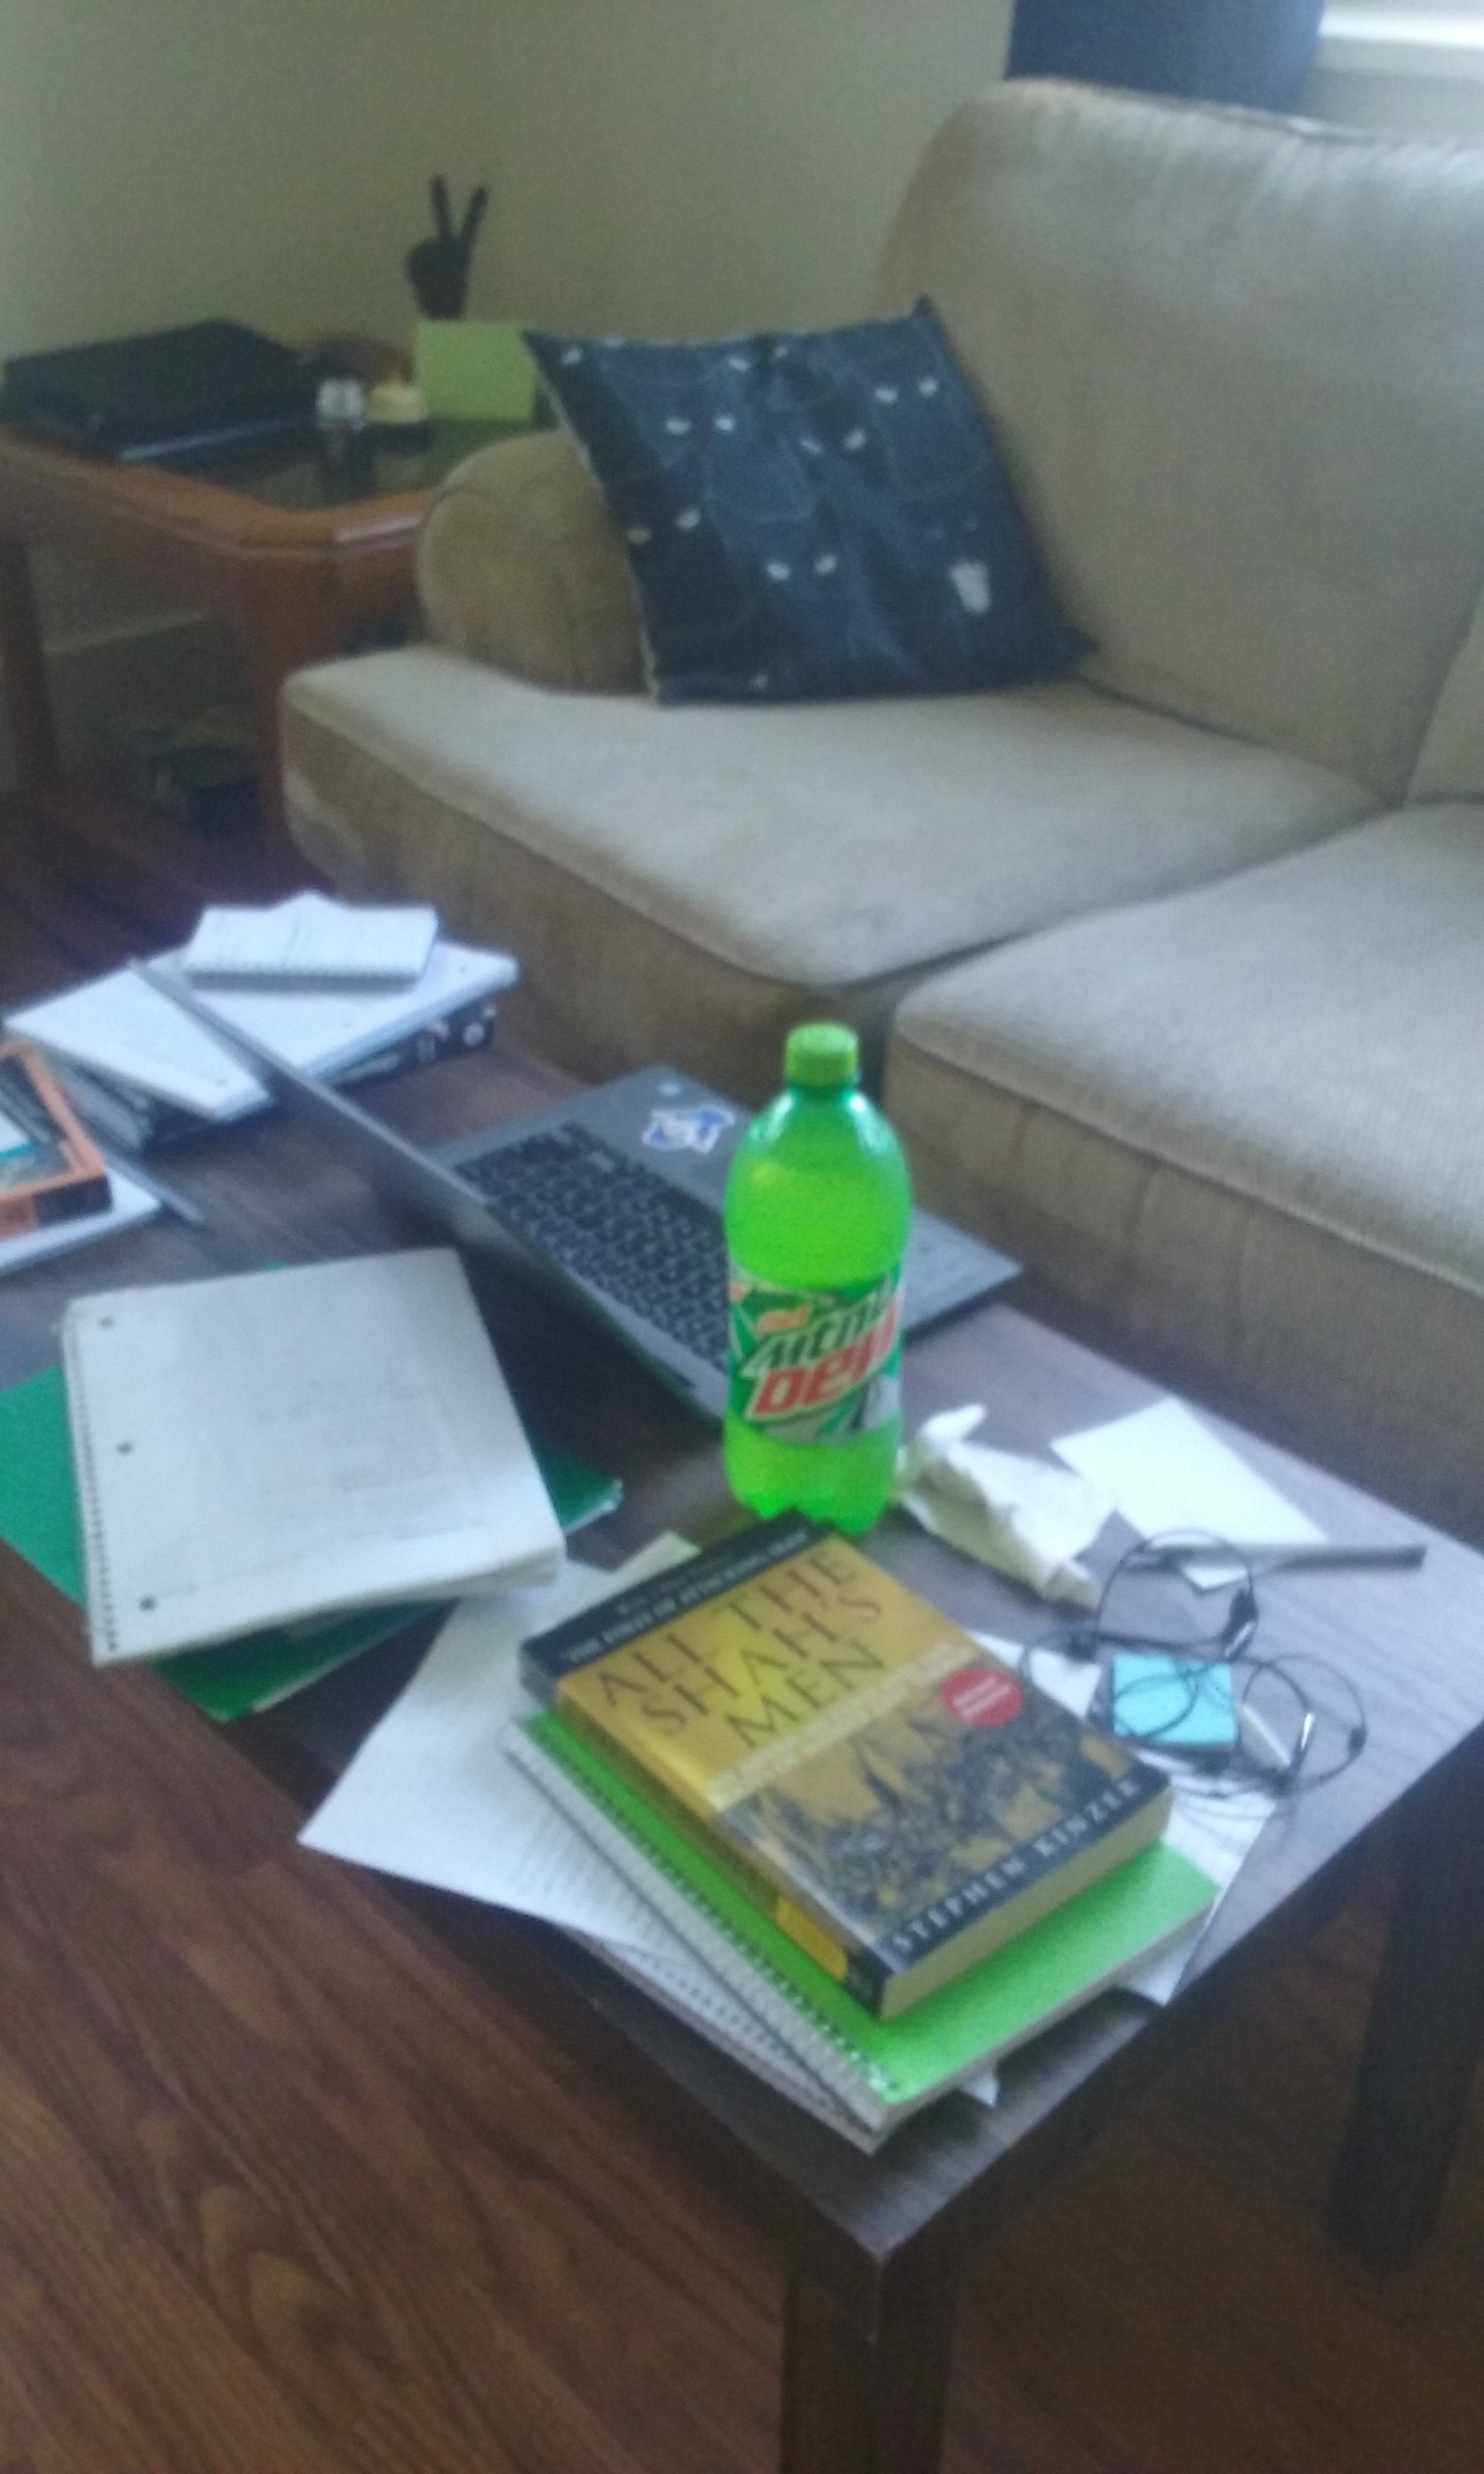
\includegraphics[width=0.4\textwidth]{coffeeTable.png}}}%
    \qquad
    \subfloat{{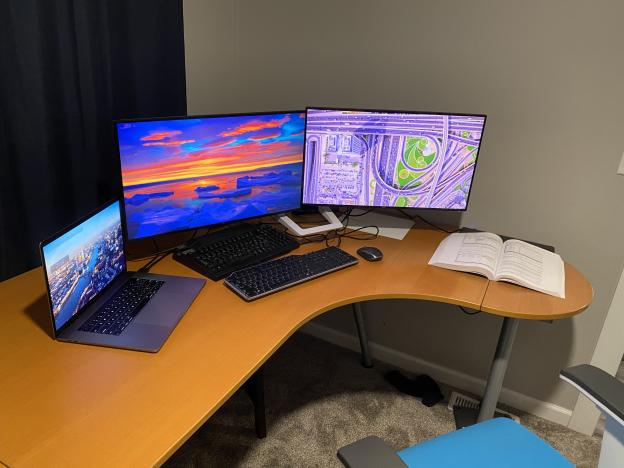
\includegraphics[width=0.4\textwidth]{goodDesk.jpg}}}%
    \caption{Varying working environments}%
    \label{fig:desks}%
\end{figure*}

\subsubsection{Socially}

This category covers the social aspects of remote learning. This category did not receive a ton of images. There was one image of someone playing a VR game; however, that image was before the pandemic. There were a few images of people in group chats.

\subsubsection{Mood}

This category covers everything that covers the mood of remote learning. This category received some of the most exciting and most depressing images. One person submitted an image of a french fry as seen in figure \ref{fig:fry} and stated: "it captures the smile you show on zoom when you're secretly dying inside because you are unmotivated and sad you have to stay inside". Remote learning has not been psychologically beneficial for students. 

\begin{figure}[h!]
    \centering
    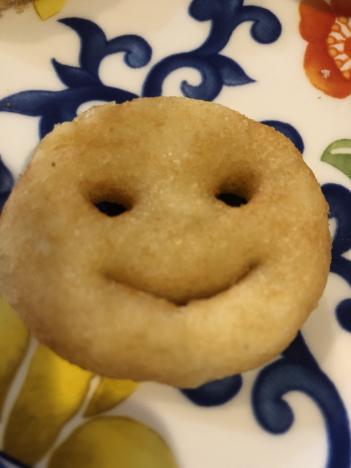
\includegraphics[width=9cm]{fry.jpg}
    \caption{Given with the caption "it captures the smile you show on zoom when you’re secretly dying inside because you are unmotivated and sad you have to stay inside"}
    \label{fig:fry}
\end{figure}


\subsection{Common Themes}

We can draw a few conclusions from both the artifact analysis and interviews. The first is the vast differences in the respondents and their different experiences as remote learners during this pandemic. Academia is supposed to be the great equalizer but, now that we are all tossed in different environments, that is no longer the case. We see that each participant had a vastly different experience with remote learning. While some people had minor difficulties with the adjustment, others saw it as a significant hurdle to jump over.


\section{Discussion}

The first thing worth mentioning is that this research is not all-encompassing. When collecting images, one alumn facetiously noted: "not a student, but I sure hope accessibility is a part of your research, especially considering the crowd RIT has." Although we did not include accessibility in this research, that is an area of potential research. Given that the researcher does not know any deaf students, conducting that accessibility research would have been challenging to initialize during social distancing-- taking an emic approach would be ideal.
Collected images and interviews were based on people that the researcher knew and who were accessible on various platforms of social interaction like Slack, Zoom, and Discord. Acknowledging this, we did not manage to interview people that were socially isolated and not a part of any friend circles. Future work can entail researching a broader scope of people. 



\subsection{Future Work}


There are two significant areas for future research questions with this realm. The first is how do we better optimize remote learning. We found that many students struggled with the transition to online learning. The second area for future work lies in how we can improve how we self isolate from each other. We are biologically wired to be social animals, so while we may do well in self-isolation in the short term, in the longer duration, we struggle to stay motivated and remain in a positive mindset. Although certain people find different coping mechanisms to help themselves be better remote learners, there is no one method works with all. A slew of factors ranging from economic, social, and mental all tie into the success of someone working remotely. We must look at how we craft public policy because it affects everyone. Remote learning was before optional, but with the pandemic, it became mandatory.


\subsection{Conclusions}

Although one may read this paper and immediately see all the negative consequences of remote learning, we must not linger on that because social distancing is essential if we are to overcome COVID-19 and future decease \cite{covidItaly}. The main takeaways from this should be the things that we should do in the future to avoid the problems that we saw when RIT did remote learning this time. The sudden decision to close the campus and go remote created a housing panic for many people. In the future, acting early on to the pandemic would have been beneficial. Many students found it hard to do remote classes in their current state. With more time to prepare for online classes, professors would be more equipped to transition their classes online in a unified, coherent fashion.

\section{Acknowledgment}

This paper got submitted as an RIT PUBL-201 project for professor Blankley's class.
The code used to generate this report can be found on the researchers Github\footnote{\url{https://github.com/jrtechs/PUBL-201-FINAL/}}.

\subsection{\label{appendix:interview}Appendix: Interview Script}


\begin{itemize}
    \item What year student are you at RIT?
    \begin{itemize}
        \item What is your major?
        \item When do you graduate?
    \end{itemize} 
    \item How have you been affected by the decision to close down campus?
    \begin{itemize}
        \item Did you have to find a new apartment? Living with family?
        \item Did you already retrieve your things from campus?
    \end{itemize}
    \item How have remote classes been going?
    \begin{itemize}
        \item Do you feel better or worse about remote learning?
        \item Did the pass/fail option lessen any stress?
        \item Do you feel like your getting enough information out of the class as compared to physical class meetings?
    \end{itemize}
    \item Where do you typically get most of your work done?
    \begin{itemize}
        \item Is it hard to get motivated to get work done?
        \item Has your sleep schedule changed?
            \begin{itemize}
                \item Are you working at weird hours?
                \item Is this a positive or negative thing for you?
            \end{itemize}
        \item Do you have more distractions when working remotely?
        \begin{itemize}
            \item internet?
            \item family?
            \item Environment (noisy neighbors, pets, etc)?
        \end{itemize}
    \end{itemize}
    \item How has doing remote classes affected you socially?
    \begin{itemize}
        \item How are your friends communicating?
        \item How are your family communicating?
        \item Are there certain people/groups of people you no-longer talk to?
        \item Has this put any stress on certain relationships?
    \end{itemize}
    \item Acknowledging that we would have to continue social distancing for at least a few more months, are there any policies that would you like to see RIT implement?
    \begin{itemize}
        \item Are teachers that make assignments open at 8:00AM and due at 9:00AM putting an undue burden on the student?
        \item Should RIT do more to help standardize the way classes are ran online or should each class be unique.
        \item Are online exams fair or accurate?
    \end{itemize}
\end{itemize}


\newpage

\bibliographystyle{plain}
\bibliography{ref}

\end{document}
